\documentclass[a4paper]{article}
%\documentclass[8pt]{report}
%%%%%%%% CREATE DOCUMENT STRUCTURE %%%%%%%%
%% Language and font encodings
\usepackage[english]{babel}
\usepackage[utf8x]{inputenc}
\usepackage[T1]{fontenc}

%\usepackage{subfig}

%% Sets page size and margins
\usepackage[a4paper,top=3cm,bottom=2cm,left=2cm,right=2cm,marginparwidth=1.75cm]{geometry}

%% Useful packages
\usepackage{amsmath}
\usepackage{graphicx}
\usepackage[colorinlistoftodos]{todonotes}
\usepackage[colorlinks=true, allcolors=blue]{hyperref}
%\usepackage{caption}
\usepackage[justification=centering]{caption}
\usepackage{subcaption}
\usepackage{sectsty}
\usepackage{float}
\usepackage{titling} 
\usepackage{blindtext}
\usepackage[square,sort,comma,numbers]{natbib}
\usepackage[colorinlistoftodos]{todonotes}
\usepackage{xcolor}
\usepackage{fancyhdr}
\usepackage{lipsum}

%% definitions 
\definecolor{darkgreen}{rgb}{0.0, 0.4, 0.0}

%% Define your personal info here %%%%%%%%%%%%%%%%%%%%%%%
\newcommand\TPid{4}
\newcommand\TPname{Ant System for Travelling Salesman Problem}
\newcommand\Firstname{Joao Filipe}
\newcommand\Familyname{Costa da Quinta}
\newcommand\Email{Joao.Costa@etu.unige.ch}

%%%%%%%%%%%%%%%%%%%%%%%%%%%%%%%%%%%%%%%%%%%%%%%%%%%%%%%

%%%%%%% Page header %%%%%%
\pagestyle{fancy}
\fancyhf{}
\rhead{TP \TPid: \TPname}
\lhead{\Firstname \Familyname}
\rfoot{Page \thepage}


%%%%%%%% DOCUMENT %%%%%%%%
\begin{document}

%%%% Title Page
\begin{titlepage}

\newcommand{\HRule}{\rule{\linewidth}{0.5mm}} 							% horizontal line and its thickness

\center 
 
% University
\textsc{\LARGE Université de Genève}\\[1cm]

% Document info
\textsc{\Large Metaheuristics for optimization}\\[0.2cm]									% Course Code
\HRule \\[0.8cm]
{ \huge \bfseries TP \TPid : \TPname}\\[0.7cm]								% Assignment
\HRule \\[2cm]
\large
\emph{Author:} \Firstname \; \Familyname\\[0.5cm]		
\emph{E-mail:} {\color{blue}\Email}\\[7cm]		
% Author info
% Author info
{\large \today}\\[2cm]

\includegraphics[width=0.4\textwidth]{images/unige_csd.png}\\[1cm] 	% University logo
\vfill 
\end{titlepage}


% ============================================
% ----------------------------------
\newpage
\section{Introduction}
During this TP we will be working on the Travelling Salesman Problem (TSP), this is a well known problem. It consists of a Salesman that is given $n$ cities/places that he has to visit, we also assume that from any city, there is a path to visit any other city with a given distance. The goal is to find the best (shortest) path such that every city is visited exactly once, this path is also called the Hamiltonian cycle of minimal length on a fully connected graph.

\section{Ant System}
Ant System (AS) is an algorithm that is designed to copy the effect of nature itself, this is what we did during the last TP as well. This time we will copy the behaviour of a group of animals, a group of ants to be more specific, hence the name of the algorithm.\\\\ Ants are not extraordinarily smart individuals, however, a group of ants is capable of incredible things. More specifically, they are capable, as a group, of finding the shortest path between their nest and a food source. Many scientific studies were done to try and understand how they were capable of such things, once we found out, we simply tried to implement the same logic into an algorithm.\\\\
What happens in nature, is that ants will randomly take a path to try and find food, at every interval of time, let's say each second, they leave behind pheromones. When new ants are coming to try and find food, they won't choose a path completely at random, they will more likely choose a path that has more pheromone, as this presence of pheromone indicates that more ants took this path than any other path.
\section{Ant System for TSP}
Let's try and apply this algorithm to TSP problem, the goal is to start the ants in one given city, and define a path as complete, if they went through each city once, and ended up at the beginning, in this analogy, the food source is in the same place as the nest. The goal is to find the shortest path that respects the conditions.\\\\ If there are $n$ cities we want to visit, a state will be a representation of which the Travelling Salesman (the Ant) visits in order. $S = [1,2,3,1]$ this state means we start at city 1, go to city 2, then 3, and finally we comeback to city 1. (We want to finish were we started). In this example n = 3, but the length of our state is 4 = n + 1. The start and end are predetermined, which means the search space is $(n-1)!$.\\\\ The total distance for a given path, is as follows : $\sum_{i = 1}^{n} D(s_{i}, s_{i+1})$ where $D(a,b)$ is the distance between city $a$ and $b$, the energy of a state will be represented by the total distance. A neighbour of a given state, is a simple city permutation in the path.\\\\
Let's see how we implement these natural mechanisms in our algorithm.\\\\
In our algorithm, a given number of ants, will try and find the best path individually, each ant attempts to find the path a certain number of times, and we goal, is that in the last iteration one of the ants finds the best path possible. The pheromone will be left at the end of an iteration, and for the next iteration the ants can make an informed decision on which path to take, based on the amount of pheromone. However, we must keep in mind that the first iteration the path is chosen at random.\\\\
\begin{itemize}
\item[(1)] Define set $J$, this set contains a list of the cities that are unvisited by a given ant. When we add a city to our path, we must delete it from $J$, which means that when $J$ is empty, the ant has found a path that respects the conditions.
\item[(2)] First task is to compute the matrix $D$ where $D_{ij}$ is the distance between cities $i$ and $j$.
\item[(3)] Compute $\eta$ where $\eta_{ij} = \frac{1}{D_{ij}}$.
\item[(4)] We create a function that returns $\tau_{ij}(t)$, this is the intensity of the path between $i$ and $j$ at iteration $t$. This intensity is the amount of pheromones.
\item[(5)] Implement a function that updates the pheromones $\tau_{ij}$. The pheromones are updated by following the next equation:\\
$$\tau_{ij}(t+1) = (1 - \rho) * \tau_{ij}(t) + \sum_{k=1}^{\#ants = m} \Delta \tau_{ij}^k(t)$$
where $\rho$ is the evaporation rate of the pheromones between each iteration, and $\Delta \tau_{ij}^k(t)$ is defined by the following equation:\\
$$\Delta \tau_{ij}^k(t) = \begin{cases} \frac{Q}{L^k(t)}$ if ant $k$ used edge $(i,j)$ in its path $\\ 0$ otherwise$ \end{cases}$$
where $Q$ is a predefined constant and $L^{k}$ is the length of the path taken by the ant. This means that a longer path will have a smaller $\frac{Q}{L^k(t)}$, which results in less pheromone for the next iterations.
\item[(6)] Finally we have to implement a function that chooses which city we visit next in our path, this is done by following the next formula:\\
$$p_{ik}^k(t) = \begin{cases} \frac{(\tau_{ij}^k(t))^{\alpha} * (\eta_{ij})^{\beta}}{\sum_{l \in J} (\tau_{il}^k(t))^{\alpha} * (\eta_{il})^{\beta}}$ if $j \in J$ $\\ 0$ otherwise$ \end{cases}$$
There are a couple of things to note in this formula. First there is a probability of 0 of choosing a city $c$ such that $c \not\in J$. Then there are the variables $\alpha$ and $ \beta$, they can be tuned to augment the importance we git to the pheromone in a given path or the visibility of a given city.
\end{itemize}
Now we simply put all the puzzle pieces together, and we have a working algorithm that copies a colony of ants.

\newpage
\section{Results}
We will run the algorithm in a unit circle of n cities, all at the same distance from the center, so the best solution is a path in shape of a circle, and then we will run the algorithm for 2 sets of cities that are given. Finally we will generate sets of larger cities, and see what happens.\\\\
For benchmark, we will use a simple greedy algorithm, this algorithm will go from city to city, always choosing the next village as the closest one that it hasn't visited yet. This algorithm is obviously deterministic. 
\begin{figure}[H]
\center
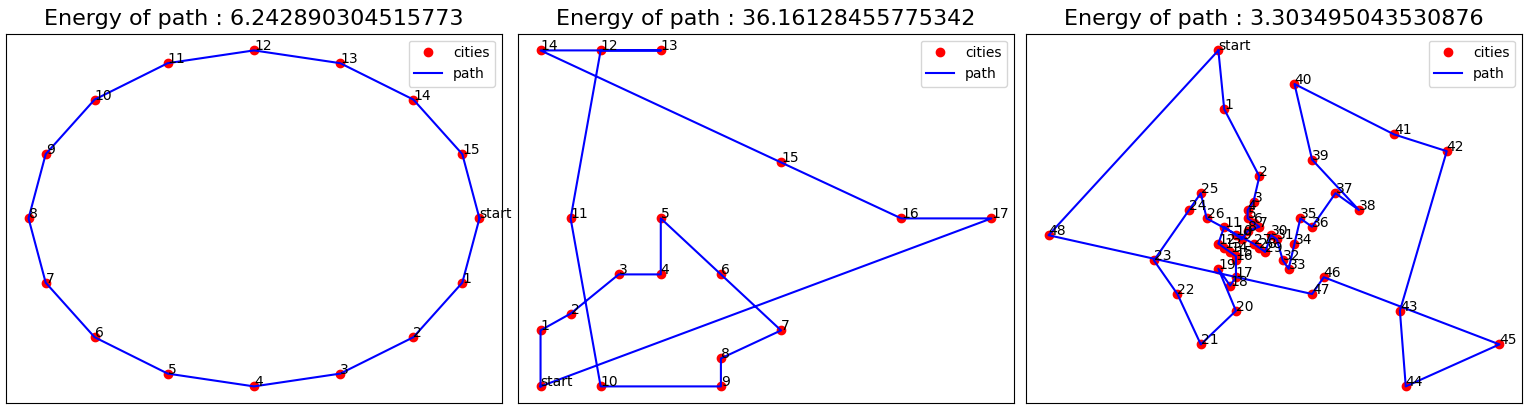
\includegraphics[width=1\textwidth]{images/algorithm_greedy.PNG}
\caption{Path found by greedy algorithm. From left to right we have : unit circle, cities.dat, cities2.dat}
\end{figure}
We can see that the algorithm only works for a perfect case scenario, and as we increase difficulty, it begins to make a mess of its path.\\\\
Let's now recall the results that we got from Simulated Annealing algorithm for the TSP problem.\\
\begin{itemize}
\item[] Unit circle mean energy for 10 runs was: 6.69
\item[] File cities.dat mean energy for 10 runs was: 28.68
\item[] File cities2.dat mean energy for 10 runs was: 2.88
\end{itemize}
\begin{center}

Random problem generator for $n = \{50, 100, 150\}$\\
\begin{tabular}{|c|c|c|c|}
\hline
        &  greedy algorithm &  SA best result &  SA mean result \\ \hline
 n = 50  &  136.10           &  115.85        &  123.65        \\ \hline
 n = 100 &  205.24           &  188.22    &  200.66         \\ \hline
 n = 150 &  243.78          &     240.92           &  259.68         \\ \hline
\end{tabular}
\end{center}

For our algorithm there are a lot of variables, some of them were imposed, and others up to us, so lets make a list of the variables and their values, as well as why (if they are not imposed):
\begin{itemize}
\item[$\alpha$] = 1 $\longrightarrow$ imposed
\item[$\beta$] = 5 $\longrightarrow$ imposed
\item[$\rho$] = 0.1 $\longrightarrow$ imposed
\item[$Q$] = $L_{nn}$ = solution determined by greedy algorithm $\longrightarrow$ imposed
\item[$\tau_0$] = $\frac{1}{L_{nn}}$ $\longrightarrow$ imposed
\item[$t_{max}$] = 5 $\longrightarrow$ not imposed. I choose this value because the algorithm wouldn't change the current best solution after the 5th iteration, for $m$ = $n^2$ 
\item[$m$] = $n^2$ $\longrightarrow$ not imposed. I choose this value because it seemed to work well with 5 iterations, this way in the first iteration we maximize the search space we visited.\\\\
\end{itemize}

\begin{figure}[H]
\center
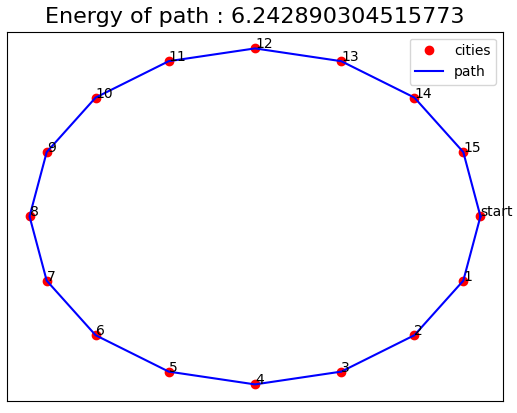
\includegraphics[width=0.5\textwidth]{images/algorithm_as_circle.PNG}
\caption{Found solution found by SA algorithm for unit circle. The energy mean for 10 runs was : 6.24}
\end{figure}

\begin{figure}[H]
\center
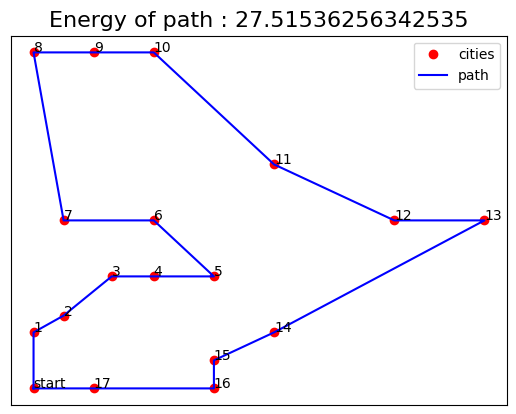
\includegraphics[width=0.5\textwidth]{images/algorithm_as_cities.PNG}
\caption{Found solution found by SA algorithm for cities.dat. The energy mean for 10 runs was : 27.51}
\end{figure}

\begin{figure}[H]
\center
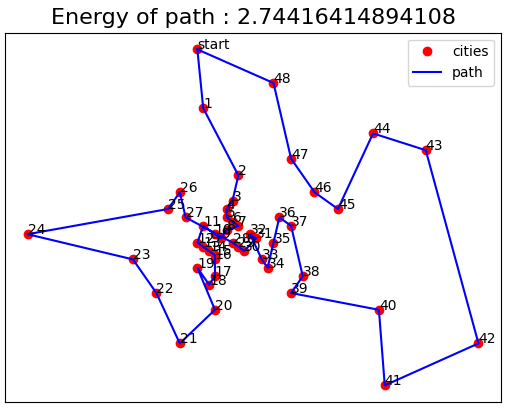
\includegraphics[width=0.5\textwidth]{images/algorithm_as_cities2.PNG}
\caption{Found solution found by SA algorithm for cities.dat. The energy mean for 10 runs was : 2.79}
\end{figure}

As we can see, Ant system performed better than Simulated annealing in every problem. However, there is a cost to this improvement, it is time, lets compare both algorithms in time:\\
\begin{center}
Time in seconds taken by both algorithms to solve each problem :\\
\begin{tabular}{|c|c|c|c|}
\hline
{\color[HTML]{000000} }                    & {\color[HTML]{000000} Unit Circle} & {\color[HTML]{000000} cities.dat} & {\color[HTML]{000000} cities2.dat} \\ \hline
{\color[HTML]{000000} Simulated Annealing} & {\color[HTML]{000000} 1.19}        & {\color[HTML]{000000} 1.47}       & {\color[HTML]{000000} 27.66}       \\ \hline
{\color[HTML]{000000} Ant System}          & {\color[HTML]{000000} 1.33}        & {\color[HTML]{000000} 2.60}       & {\color[HTML]{000000} 116.01}      \\ \hline
\end{tabular}
\end{center}
We can easily see that there is a cost associated with the better results fond by Ant System .. \\\\
We could obviously argue that if we change the parameter $m$ we would have a faster algorithm, but then it wouldn't be as good, and if it isn't as good, then there is less incentive to use it over Simulated Annealing.\\\\
For the final part of this results section, we will generate random problems of size $n = \{20, 40, 60, 80, 100\}$, and run each problem 10 times, and compare it to a greedy implementation. However, as the parameter $m=n^2$, it will just be too large, and take too much time, so for the purpose of these simulations I will set $m=10*n$.

\begin{center}
Energy for each randomly generated problem, the AS result is the mean of 10 attempts at the same problem :\\
\begin{tabular}{|c|c|c|c|c|c|}
\hline
{\color[HTML]{000000} }           & {\color[HTML]{000000} 20}     & {\color[HTML]{000000} 40}     & {\color[HTML]{000000} 60}     & 80     & 100    \\ \hline
{\color[HTML]{000000} Greedy}     & {\color[HTML]{000000} 100.42} & {\color[HTML]{000000} 120.81} & {\color[HTML]{000000} 143.66} & 199.74 & 205.69 \\ \hline
{\color[HTML]{000000} Ant System} & {\color[HTML]{000000} 84.48}  & {\color[HTML]{000000} 104.55} & {\color[HTML]{000000} 133.22} & 155.94 & 174.65 \\ \hline
\end{tabular}
\end{center}
Ant system performed better than Greedy, as expected, even with $m=10*n$. If we go back and look at the results of SA, we see that even with $m=10*n$ AS performed better than SA for the randomly generated problems. 
\end{document}
